%% The following is a directive for TeXShop to indicate the main file
%%!TEX root = diss.tex

\chapter{Introduction}
\label{ch:Introduction}

%%%%%%%%%%%%%%%%%%%%%%%%%%%%%%%%%%%%%%%%%%%%%%%%%%%%%%%%%%%%%%%%%%%%%%
\section{Motivation}

Since the neutrino was first postulated by Wolfgang Pauli in 1930 \cite{neutrinoHistory}, neutrinos have proven to be an important probe into various fundamental properties of our universe.
Because neutrinos do not react via the electromagnetic or strong force, they may only be detected via the weak force, presenting a significant challenge to any attempts to measure them.
Over the past 60 years, physicists have built increasingly sophisticated and sensitive detectors to accurately measure the properties of these particles.

There are three flavors of neutrinos: the electron neutrino $\nu_e$, the muon neutrino $\nu_\mu$, and the tau neutrino $\nu_\tau$.
The flavor of the neutrino determines what interactions it might have.
In 1998, the Super-Kamiokande detector in Japan observed clear evidence of neutrino oscillation: as neutrinos of one flavor travels over a large distance, it has some probability of later being observed as a neutrino of another generation.
This implied that neutrinos have a nonzero mass, a result not predicted by the Standard Model.
The theorized explanation for neutrino oscillation is that each neutrino flavor actually exists as some superposition of 3 different mass states. As a neutrino travels over large distances, the differences in phases of the mass states results in a shifting probability of detecting each neutrino flavor.
The relationship between mass and flavor states is governed by the following relation:

\[
\begin{pmatrix}
\nu_e \\ \nu_\mu \\ \nu_\tau
\end{pmatrix}
=
%U
\begin{pmatrix}
U_{e1} & U_{e1} & U_{e1} \\ 
U_{\mu 1} & U_{\mu 2} & U_{\mu 3} \\
U_{\tau 1} & U_{\tau 2} & U_{\tau 3}
\end{pmatrix}
\begin{pmatrix}
\nu_1 \\ \nu_2 \\ \nu_3
\end{pmatrix}
\]


Here, U is a $3 \times 3$ unitary matrix, known as the Pontecorvo–Maki–Nakagawa–Sakata (PMNS) Matrix. The matrix can be characterized by 4 parameters: $\theta_{12}, \theta_{23}$, and $\theta_{13}$, which are the mixing angles, and $\delta_{CP}$, known as the CP-violating phase \cite{pdg2018}. The probability of a neutrino oscillating from one flavor to another is governed by the distance travelled, the mixing angles, and $\Delta m_{ij}^2$, the squared mass difference between neutrino states. 


There are many open-ended questions regarding neutrinos.
The mixing angles of the PMNS matrix and the squared mass differences remain to be more accurately measured.
Because only the differences in masses are known, the actual ordering and absolute values of the masses are unknown.
It is unknown whether neutrinos are their own anti-particles (i.e. whether the neutrino is a Majorana fermion), or if the antineutrino is a distinct particle (i.e. a Dirac fermion).
It is uncertain whether $\sin(\delta_{CP})$ is consistent with zero: If it is nonzero, then that may explain the asymmetry between the amount of matter and antimatter in the universe \cite{neutrinoCP}.

The next generation of neutrino experiments aim to answer all of these questions (and more) to a high degree of precision - they include the Deep Underground Neutrino Experiment (DUNE) \cite{duneDesign} and the Hyper-Kamiokande experiment \cite{hyperKDesign}.
In both experiments, a large flux of neutrinos is generated with a particle accelerator hundreds of kilometers away from a large neutrino detector.
When a sufficiently energetic particle beam hits a target, the collision produces secondary particles: mostly charged pions and kaons.
Magnetic horns are used to direct these secondary particles in the direction of the distant detector.
The charged pions will decay in flight as follows:

$$ \pi^+ \rightarrow \mu^+ + \nu_\mu \quad   \text{and} \quad \mu^+ \rightarrow \bar{\nu}_e + \nu_\mu$$

The charged kaons have several decay modes, but the most common are:

$$ K^+ \rightarrow \mu^+ + \nu_\mu \text{,} \quad  K^+ \rightarrow \pi^+ + \pi^0  \text{,}\quad K^+ \rightarrow \pi^0 + e^+ + \nu_e$$

There are corresponding charge-conjugate decays for the $\pi^-$ and $K^-$. 
As these secondary particles decay, a large number of resulting neutrinos are sent in the direction of the detector, where only a very small fraction will be detected.

These next-generation neutrino experiments have a far higher level of statistics than in neutrino experiments of the past, due to the massive size of the detectors.
Because the error is no longer dominated by statistical error, decreasing any systematic error is increasingly important.
In such experiments, the two major sources of systematic error arises from uncertainty in the neutrino-nucleus interaction, and uncertainty in calculations of the neutrino flux.
The primary contribution to the uncertainty of neutrino flux lies in uncertainty in the hadron production \cite{hyperKDesign}.

The NA61/SHINE experiment, located at CERN, has been very successful in measuring hadron production resulting from collisions of particles from the Super Proton Synchrotron onto various targets \cite{na61}.
These measurements significantly reduced neutrino flux uncertainties in T2K, an ongoing accelerator-based neutrino oscillation experiment \cite{na61T2K}. 
However, the momenta of the measured beams are constrained to between 13 and 160 GeV/c.
This does not allow for the calculations of low-momentum hadron reinteractions: in addition to hadrons directly decaying into neutrinos, some hadrons may reinteract with the target, magnetic horns, or beamline of the detector, affecting the neutrino flux.
Furthermore, some neutrino experiments aim to measure atmospheric neutrinos (neutrinos resulting from the decay of products of the reaction of cosmic rays with the atmosphere), and the NA61/SHINE data does not cover the associated lower-momentum hadron interactions.

 \section{\ac{EMPHATIC}}

In order to constrain hadron production uncertainties, work is in progress for EMPHATIC (Experiment Measuring the Production of Hadrons At a Test-beam In Chicagoland).
EMPHATIC is a tabletop experiment designed to precisely measure hadron interactions resulting from a proton or pion beam impinging on various targets. 
EMPHATIC is located at the Fermilab Test Beam Facility, and the proposed experimental setup is shown in Figure \ref{fig:EMPHATIC}.
The Fermilab Test Beam can produce a beam with momenta ranging from 0.2-120 GeV, which complements the momenta measured by NA61/SHINE.

\begin{figure}[] 
\centering
\resizebox{0.75\textwidth}{!}{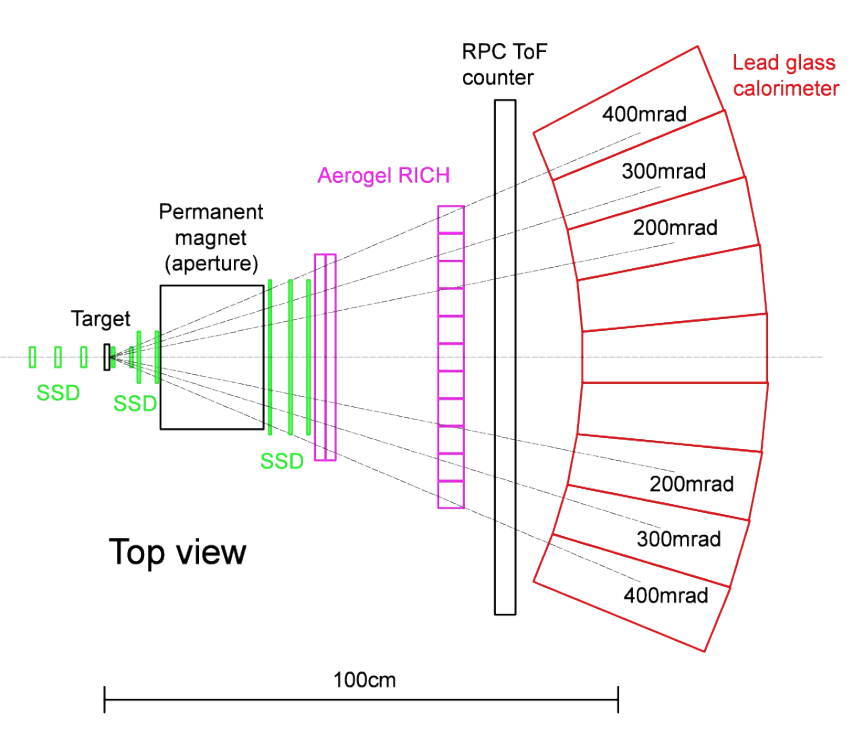
\includegraphics{./figs/EMPHATIC.png}}
\caption[Top view of the proposed EMPHATIC setup]{Top view of the proposed EMPHATIC setup, obtained with permission from the EMPHATIC group. The different detectors in the setup are shown in different colours.}
\label{fig:EMPHATIC} 
\end{figure}

To obtain measurements for accelerator-based neutrino experiments, \ac{EMPHATIC} will measure targets of graphite, aluminum, and iron.
These targets correspond to the composition of the proposed targets, magnetic horns, and beamline components typically found in accelerator-based neutrino experiments.
\ac{EMPHATIC} will also measure targets composed of boron, boron nitride, and boron trioxide.
Because the atmosphere is primarily composed of nitrogen and oxygen, measuring the latter two targets and removing the effects of pure boron will lead to an estimation of hadron production arising from the interaction of cosmic rays in the atmosphere. 

\ac{EMPHATIC} includes four different kinds of detectors that serve to measure hadron production.
A set of silicon strip detectors (SSDs) register the position of each particle as they pass through.
A permanent magnet downstream of the target causes the trajectory of particles to curve due to the Lorentz force: the radius of the curvature is proportional to momentum of the particle, so using multiple SSDs downstream of the magnet allows for the measurement of particle momenta and trajectories.
The particles then pass through an Aerogel Ring Imaging Cherenkov (ARICH) detector.
As explained in Section \ref{sec:ARICH}, this detector can be used to determine a charged particle's velocity if its trajectory is known. 
If the velocity and momentum of a particle are known, then its mass may be determined.
This allows for the identification of each particle. 

After passing through the ARICH detector, particles will pass through a resistive plate chamber time-of-flight (RPC ToF) detector.
This detector measures the time at which a particle passes through and compares this to an upstream measurement, giving another measure of velocity. 
Unlike the ARICH detector, the ToF detector does not have the resolution sufficient to properly identify forward-angle high-momentum particles, but due to its greater angular coverage, it is able to identify lower-momentum particles.
These two detectors complement each other to provide a full measurement of velocities across a broad range.
Following this, particles strike a lead glass calorimeter, which measures the final particle energy.
The lead glass calorimeter is useful for identifying electrons or neutrons.

\section{Overview of the project}
Development is underway on the simulation and design of the ARICH detector for EMPHATIC.
The ARICH detector should be able to accurately distinguish between charged pions, charged kaons, and protons over a broad spectrum of momenta.
We propose to use the ARICH detector to conduct particle identification by using a likelihood approach. 
With this approach, photon measurements from each experimental event is compared against several different Monte Carlo simulations of that event, each representing a different hypothesis for what particle or particles were involved.
The particle or particles that produced the simulated distribution that best matches the experimental data is then chosen as the most likely candidate.
This technique is fully described in Chapter \ref{sec:particleIdentification}. 

Concurrent work is underway for a full end-to-end Monte Carlo simulation of the EMPHATIC experimental setup.
This simulation is created using Geant4, a platform designed for Monte Carlo simulations of particles passing through matter \cite{geant4}.
This simulation will contain information on the placement of all detector components and their materials, and models the physical interactions of each particle running through the experiment, and the shower of secondary particles produced.
While the Geant4 simulation should give accurate results for the distribution of optical photons for different particle hypotheses, it is relatively slow to perform for each particle.
Using this likelihood approach to particle identification, we would be required to run several different simulations per experimental event.
The Geant4 simulation is therefore too slow to be run as a tool for particle identification, necessitating the need for a more efficient fast simulation of just the optical processes in the ARICH detector. 

In this project, I created such a fast simulation that incorporates the necessary physical processes while maintaining high efficiency.
%The outputs of this simulation are then compared to the full Geant4 simulation.
The simulation is described in Chapter \ref{ch:Methods}.
Following this, the particle identification performance of this technique was evaluated under several different conditions.
The particle identification and its evaluation are described in Chapter \ref{ch:Results}.

\endinput

Any text after an \endinput is ignored.
You could put scraps here or things in progress.
